\documentclass[12pt]{article}
\usepackage[printonlyused,withpage]{acronym} % acronyms
\usepackage{amsmath}
\usepackage{amssymb}
\usepackage{amsthm}
\usepackage[page,title,toc]{appendix} % appendix
\usepackage{array} % tables (?)
\usepackage{bbold} % \mathbb
\usepackage[backend=biber, style=apa]{biblatex} % bibliography
\usepackage{bm} % bold math
\usepackage{caption} % better captioning and figure numbering (?)
\usepackage{changepage} % some landscape pages
\usepackage{csquotes} % \blockquote
\usepackage{enumitem} % control spacing
\usepackage{etoolbox} % for a macro (?)
\usepackage{fancyhdr}				% For fancy header/footer
\usepackage{float}      % use the [H] option for positioning
\usepackage[T1]{fontenc}
\usepackage{fontspec}
\usepackage[hang,flushmargin]{footmisc} % don't indent footnotes
\usepackage{gensymb} % \degree symbol
\usepackage{glossaries} % glossary
\usepackage{graphicx}				% For including figure/image
\usepackage[margin=1.0in,includehead,includefoot]{geometry}		% For setting margins
\usepackage{import}    % \incfig
\usepackage[iso,american]{isodate}
\usepackage{makecell}  % multi-row table cells
%\usepackage{mathptmx}  % make math Times New Roman
%\usepackage{minted}    % code styling
\usepackage{pdflscape} % make \incfig to landscape
\usepackage{pdfpages} % \includepdf
%\usepackage{pgffor} % iterate over the modular files to import their labels
\usepackage{pgfplots} % bar chart
\usepackage{ragged2e} % \raggedright
\usepackage{setspace} % {single,one-half}space \doublespacing
\usepackage{soul} % underline across line breaks
\usepackage{svg}
\usepackage{textcomp} % textcomp to get rid of gensymb warnings
%\usepackage{times} % Times New Roman, only pdflatex
\usepackage{transparent} % \incfig (breaks pgffor)
\usepackage[normalem]{ulem} % allow \smash of underlines
\usepackage{vcell} % vertical writing in table cells (?)
\usepackage{wrapfig} % \incfig
\usepackage{xifthen} % \incfig
\usepackage{xparse} % ?
\usepackage{xr} % ?

% hYpErReF mUsT cOmE lAsT
\usepackage[hidelinks]{hyperref} % \href{url}{text}
\hypersetup{colorlinks=true,linkcolor=black,urlcolor=blue,filecolor=black,citecolor=black}

% svg and Inkscape's pdf_tex
\newcommand{\incfig}[2]{
	\def\svgwidth{#1\columnwidth}
	\import{./}{#2.pdf_tex}
}

% Bibliography
%\addbibresource{}

% Font size reminder
% \tiny \small \normalsize \large \Large \Huge
%\setmainfont{Times New Roman}
\setmonofont{Mononoki Nerd Font Mono}[Scale=MatchLowercase]

%%% Macros
% Horizontal Spacing
\newcommand\hs{\hspace{1cm}}
\newcommand\hhs{\hspace{0.5cm}}
% Singlespacing in certain environments: \ssInEnv{environment, font=\normalsize}
% \newcommand{\ssInEnv}[2][\normalsize]{\BeforeBeginEnvironment{#2}{\begin{singlespace*}{#1}}\AfterEndEnvironment{#2}{\end{singlespace*}}}
% Fancy header and footer for homeworks
\newcommand\hwheadfoot{
\pagestyle{fancy}
\fancyhead[LO,L]{Lorenzo Hess}
\fancyhead[CO,C]{CLASS: Homework NUMBER} % TODO
\fancyhead[RO,R]{\today} % TODO
%\fancyfoot[LO,L]{}
\fancyfoot[CO,C]{\thepage}
%\fancyfoot[RO,R]{}
\topmargin=-0.75in
\renewcommand{\headrulewidth}{0.4pt}
\renewcommand{\footrulewidth}{0.4pt}}

% Homework problems with arbitrary numbers without worrying about section formatting and counters
\newcommand{\problemSection}[1]{ % Args = section number
\noindent\Large\textbf{Section #1}
}
\newcommand{\problem}[1]{ % Args = number
\noindent\large\textbf{Problem #1}
}

% Volume symbol (heat transfer)
\newcommand{\volume}{{\ooalign{\hfil$V$\hfil\cr\kern0.08em--\hfil\cr}}}

% Table of Contents tweaks
% Singlespacing
\let\oldToC\tableofcontents
\renewcommand{\tableofcontents}{\begin{singlespace}\oldToC\end{singlespace}}
% Include subsubsections
\setcounter{tocdepth}{3}

% Spacing
\singlespacing
% \ssInEnv{itemize}
% \ssInEnv{enumerate}
% \ssInEnv{tabular}
\setlist{listparindent=\parindent, % indent paragraphs under \item
  nolistsep} % no spacing between list items

% Smash underlines
\let\oldunderline\underline
\renewcommand{\underline}[1]{\oldunderline{\smash{#1}}}
\setlength\ULdepth{1.5pt}

% Minted code styling
%\usemintedstyle{friendly}
%\setminted[matlab]{fontsize=\normalsize, breaklines=true, breakanywhere=true, linenos=true, numbersep=6pt, stripnl=true, baselinestretch=1}
%\setminted[text]{fontsize=\scriptsize, breaklines=true, breakanywhere=true, linenos=false, numbersep=6pt, stripnl=true, baselinestretch=1}

\author{Lorenzo Hess}
\date{\today}
\title{Homework 1: Linkage Analysis}

\begin{document}
\maketitle
\tableofcontents

\newpage
\section{Assumptions}%
\label{assum}

\begin{enumerate}
  \item Steady-state rate of 7450 parts in seven hours
  \item Links made of 7075 Aluminum
  \item Link geometry: 10cm width, 5cm thickness, 6cm joint diameter
  \item Negligible gripper weight
  \item Ideal revolute joints, e.g. no friction, only one DOF
  \item Ideal links, e.g. no deformation, fatigue
  \item Constant input angular velocity
\end{enumerate}

\section{Schematics}%
\label{schematics}

The kinematic outline of the six-bar linkage is shown in Figure \ref{fig:kin-outline}. Recall that link FG extends beyond joint F to accommodate a gripper.

\begin{figure}[H]
  \centering
  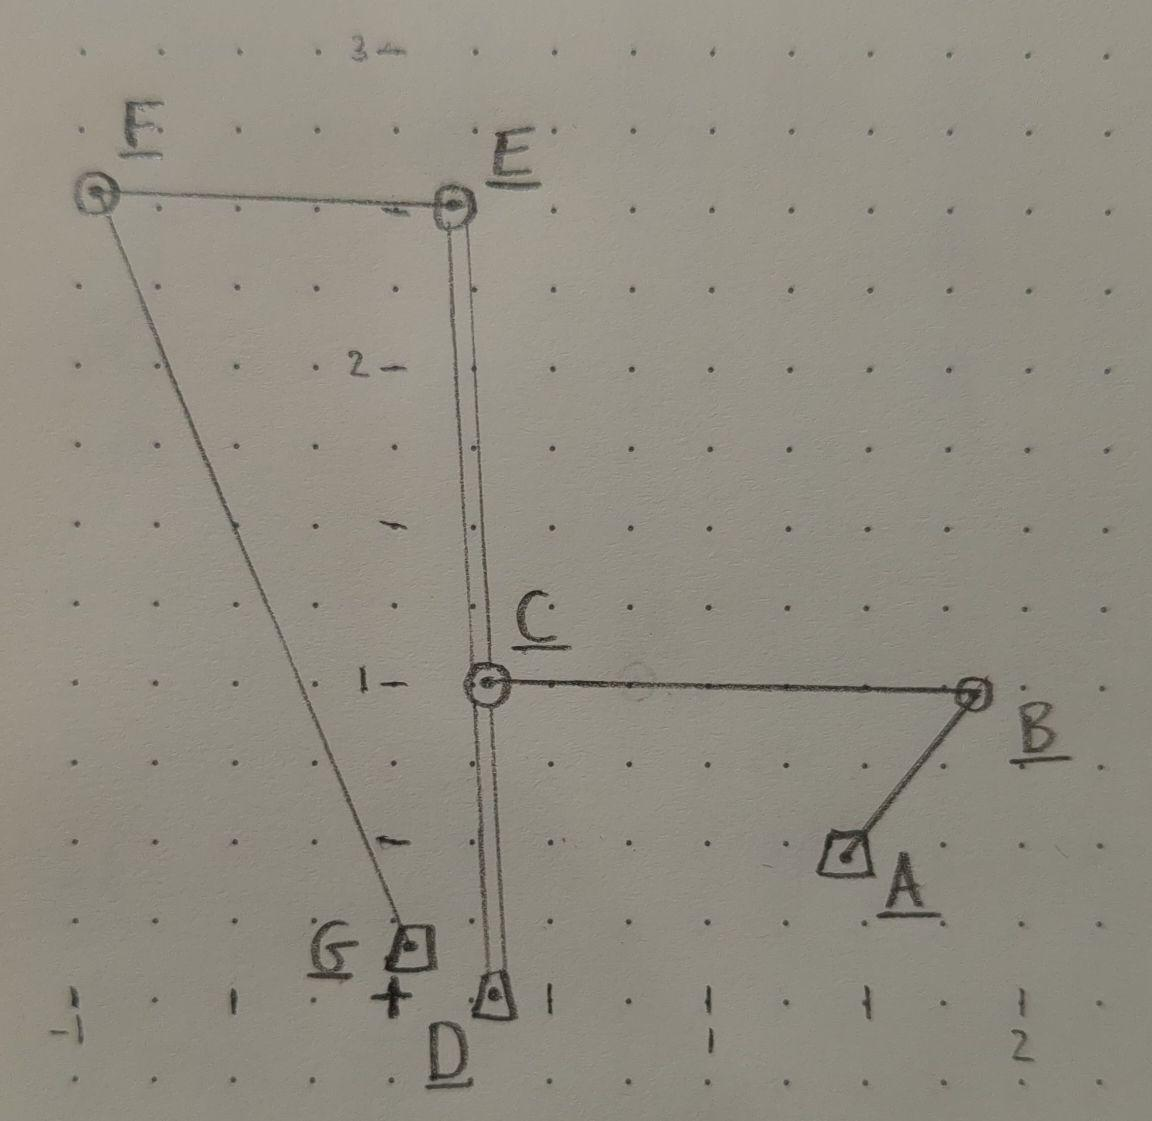
\includegraphics[scale=0.25]{../kinematic-outline.jpeg}
  \caption{\label{fig:kin-outline}Kinematic outline of the linkage.}
\end{figure}

A free-body diagram of each link is shown in Figure \ref{fig:fbds}, with an input torque $\tau_{\text{in}}$, weights $W$, at center of masses $s$, and with artifact weight $W_{\text{art}}$.

\begin{figure}[H]
  \centering
  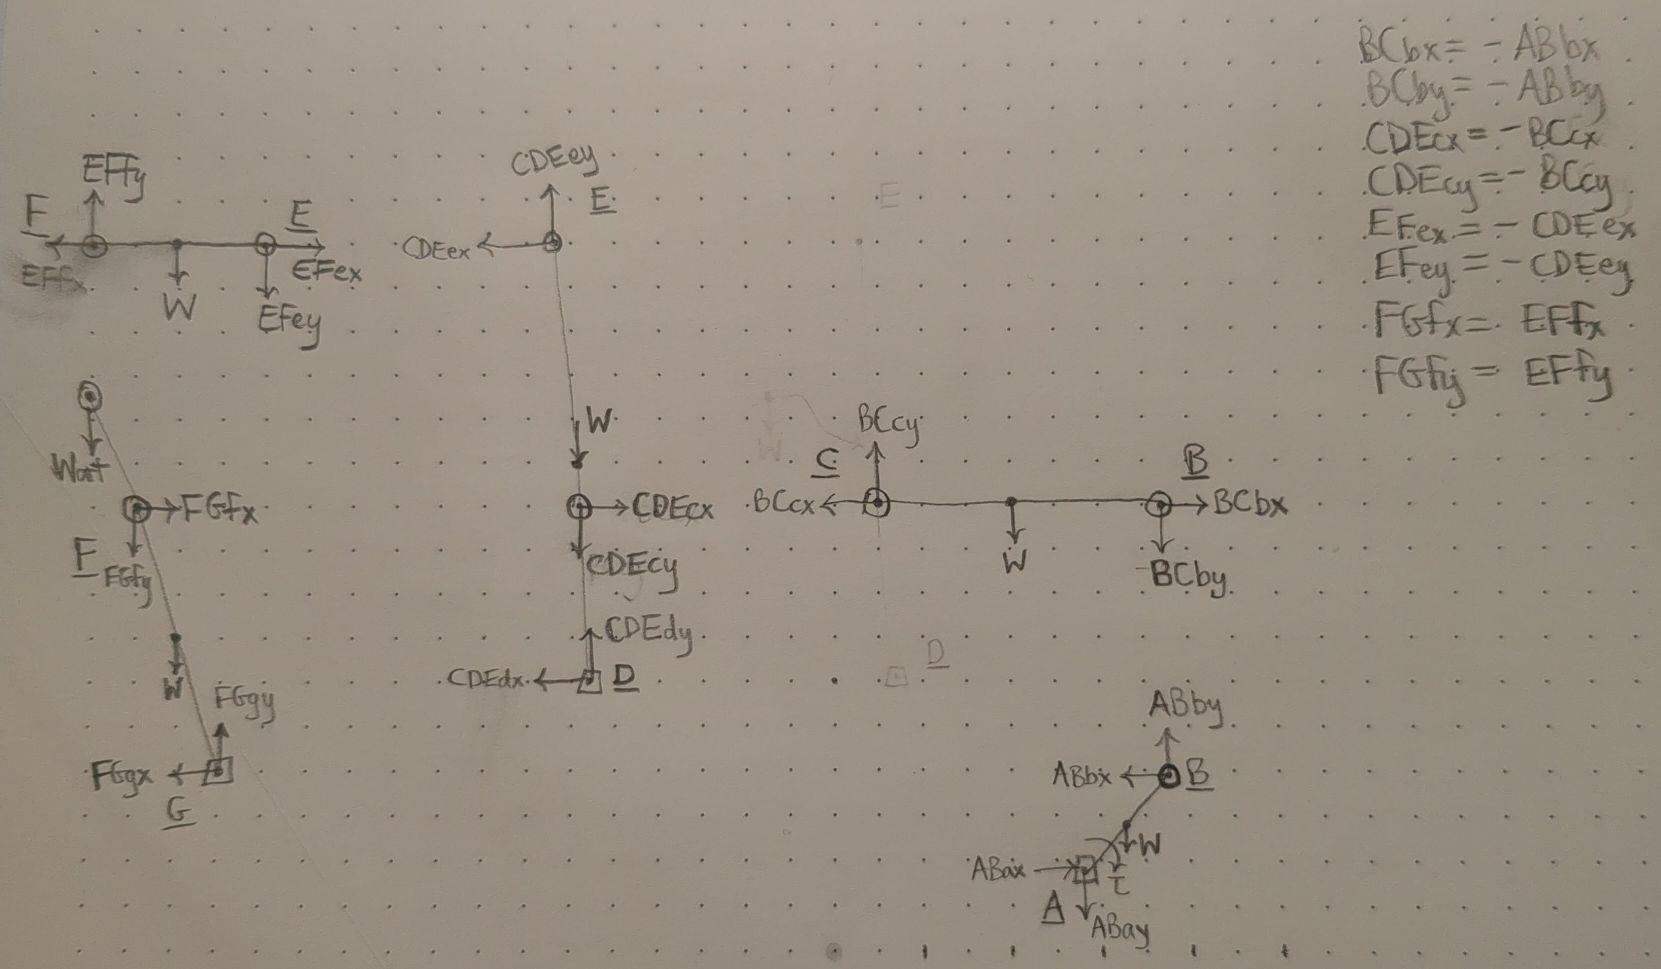
\includegraphics[scale=0.3]{../fbds.jpeg}
  \caption{\label{fig:fbds}Free-body diagram of each link.}
\end{figure}

\section{Statics and Dynamics Equations}%
\label{eqns}

\subsection{Forces and Moments}%
\label{eqns.forces-moments}

\subsubsection{Static Equilibrium}%
\label{eqns.forces-moments.static}

At static equilibrium, the net force and moment on each link is zero. Each link yields one vector force equation; link AB also yields one vector moment equation. All force equations have two components, and the moment equation has three components.

For link AB, with moments about joint A:
\[ R_{a,x} - R_{b,x} = 0 \hs -R_{a,y} + R_{b,y} - W_{ab} = 0 \hs \vec{\tau}_{in} + \vec{r}_{s/a}\times \vec{W}_{ab} + \vec{r}_{b/a}\times \vec{R}_{b} = 0 \]
For link BC, with moments about joint B:
\[ R_{b,x} - R_{c,x} = 0 \hs -R_{b,y} + R_{c,y} - W_{bc} = 0 \hs \vec{r}_{s/b}\times \vec{W}_{bc} + \vec{r}_{c/b}\times \vec{R}_{c} = 0 \]
For link CDE, with moments about joint C:
\[ R_{d,x} - R_{c,x} - R_{e,x} = 0 \hs R_{d,y} - R_{c,y} - R_{e,y} - W_{cde} = 0 \hs \vec{r}_{s/c}\times \vec{W}_{cde} + \vec{r}_{e/c}\times \vec{R}_{e} + \vec{r}_{d/c}\times \vec{R}_{d} = 0 \]
For link EF, with moments about joint E:
\[ R_{e,x} - R_{f,x} = 0 \hs -R_{e,y} + R_{f,y} - W_{ef} = 0 \hs \vec{r}_{s/e}\times \vec{W}_{ef} + \vec{r}_{f/e}\times \vec{R}_{f} = 0 \]
For link FG, with moments about joint G:
\[ R_{f,x} - R_{g,x} = 0 \hs -R_{f,y} + R_{g,y} - W_{fg} - W_{\text{art}} = 0 \hs \vec{r}_{s/g}\times \vec{W}_{fg} + \vec{r}_{f/g}\times \vec{R}_{f} + \vec{r}_{\text{art}/g}\times \vec{W}_{\text{art}} = 0 \]

\subsubsection{Dynamic Equilibrium}%
\label{eqns.forces-moments.dynamic}

The dynamic equilibrium for each link is given by Newton's Second Law at the center of mass:
\[ \Sigma \vec{F} = M \vec{a}_{s} \]
For rotational dynamics about joint $i$:
\[ \Sigma \vec{T}_{i} = J_{i} \vec{\alpha} \]
We will compute the net force and torque on each link by computing $M \vec{a}_{s}$ or $J \vec{\alpha}$ after having calculated the respective accelerations.

\subsection{Mass Calculations}%
\label{eqns.masses}

All links were modeled in Onshape with material of Aluminum 7075. For all binary links, I placed the centroid of the flat face at the origin and used a symmetric extrude to ensure the center of mass also coincides with the origin. Link FG was extended by 1.843m beyond joint F and uses the same rounded end, with a pin for the gripper. For link CDE, joint D is placed at the origin and joint C at 0.98m distance away.  Link AB is shown in Figure \ref{fig:link-AB-CAD}. The joint-to-joint center distance was varied to produce different links. The mass properties were computed with Onshape's ``Mass and Section Properties'' feature and are in Table \ref{tab:link-masses}.

\begin{figure}[ht]
  \centering
  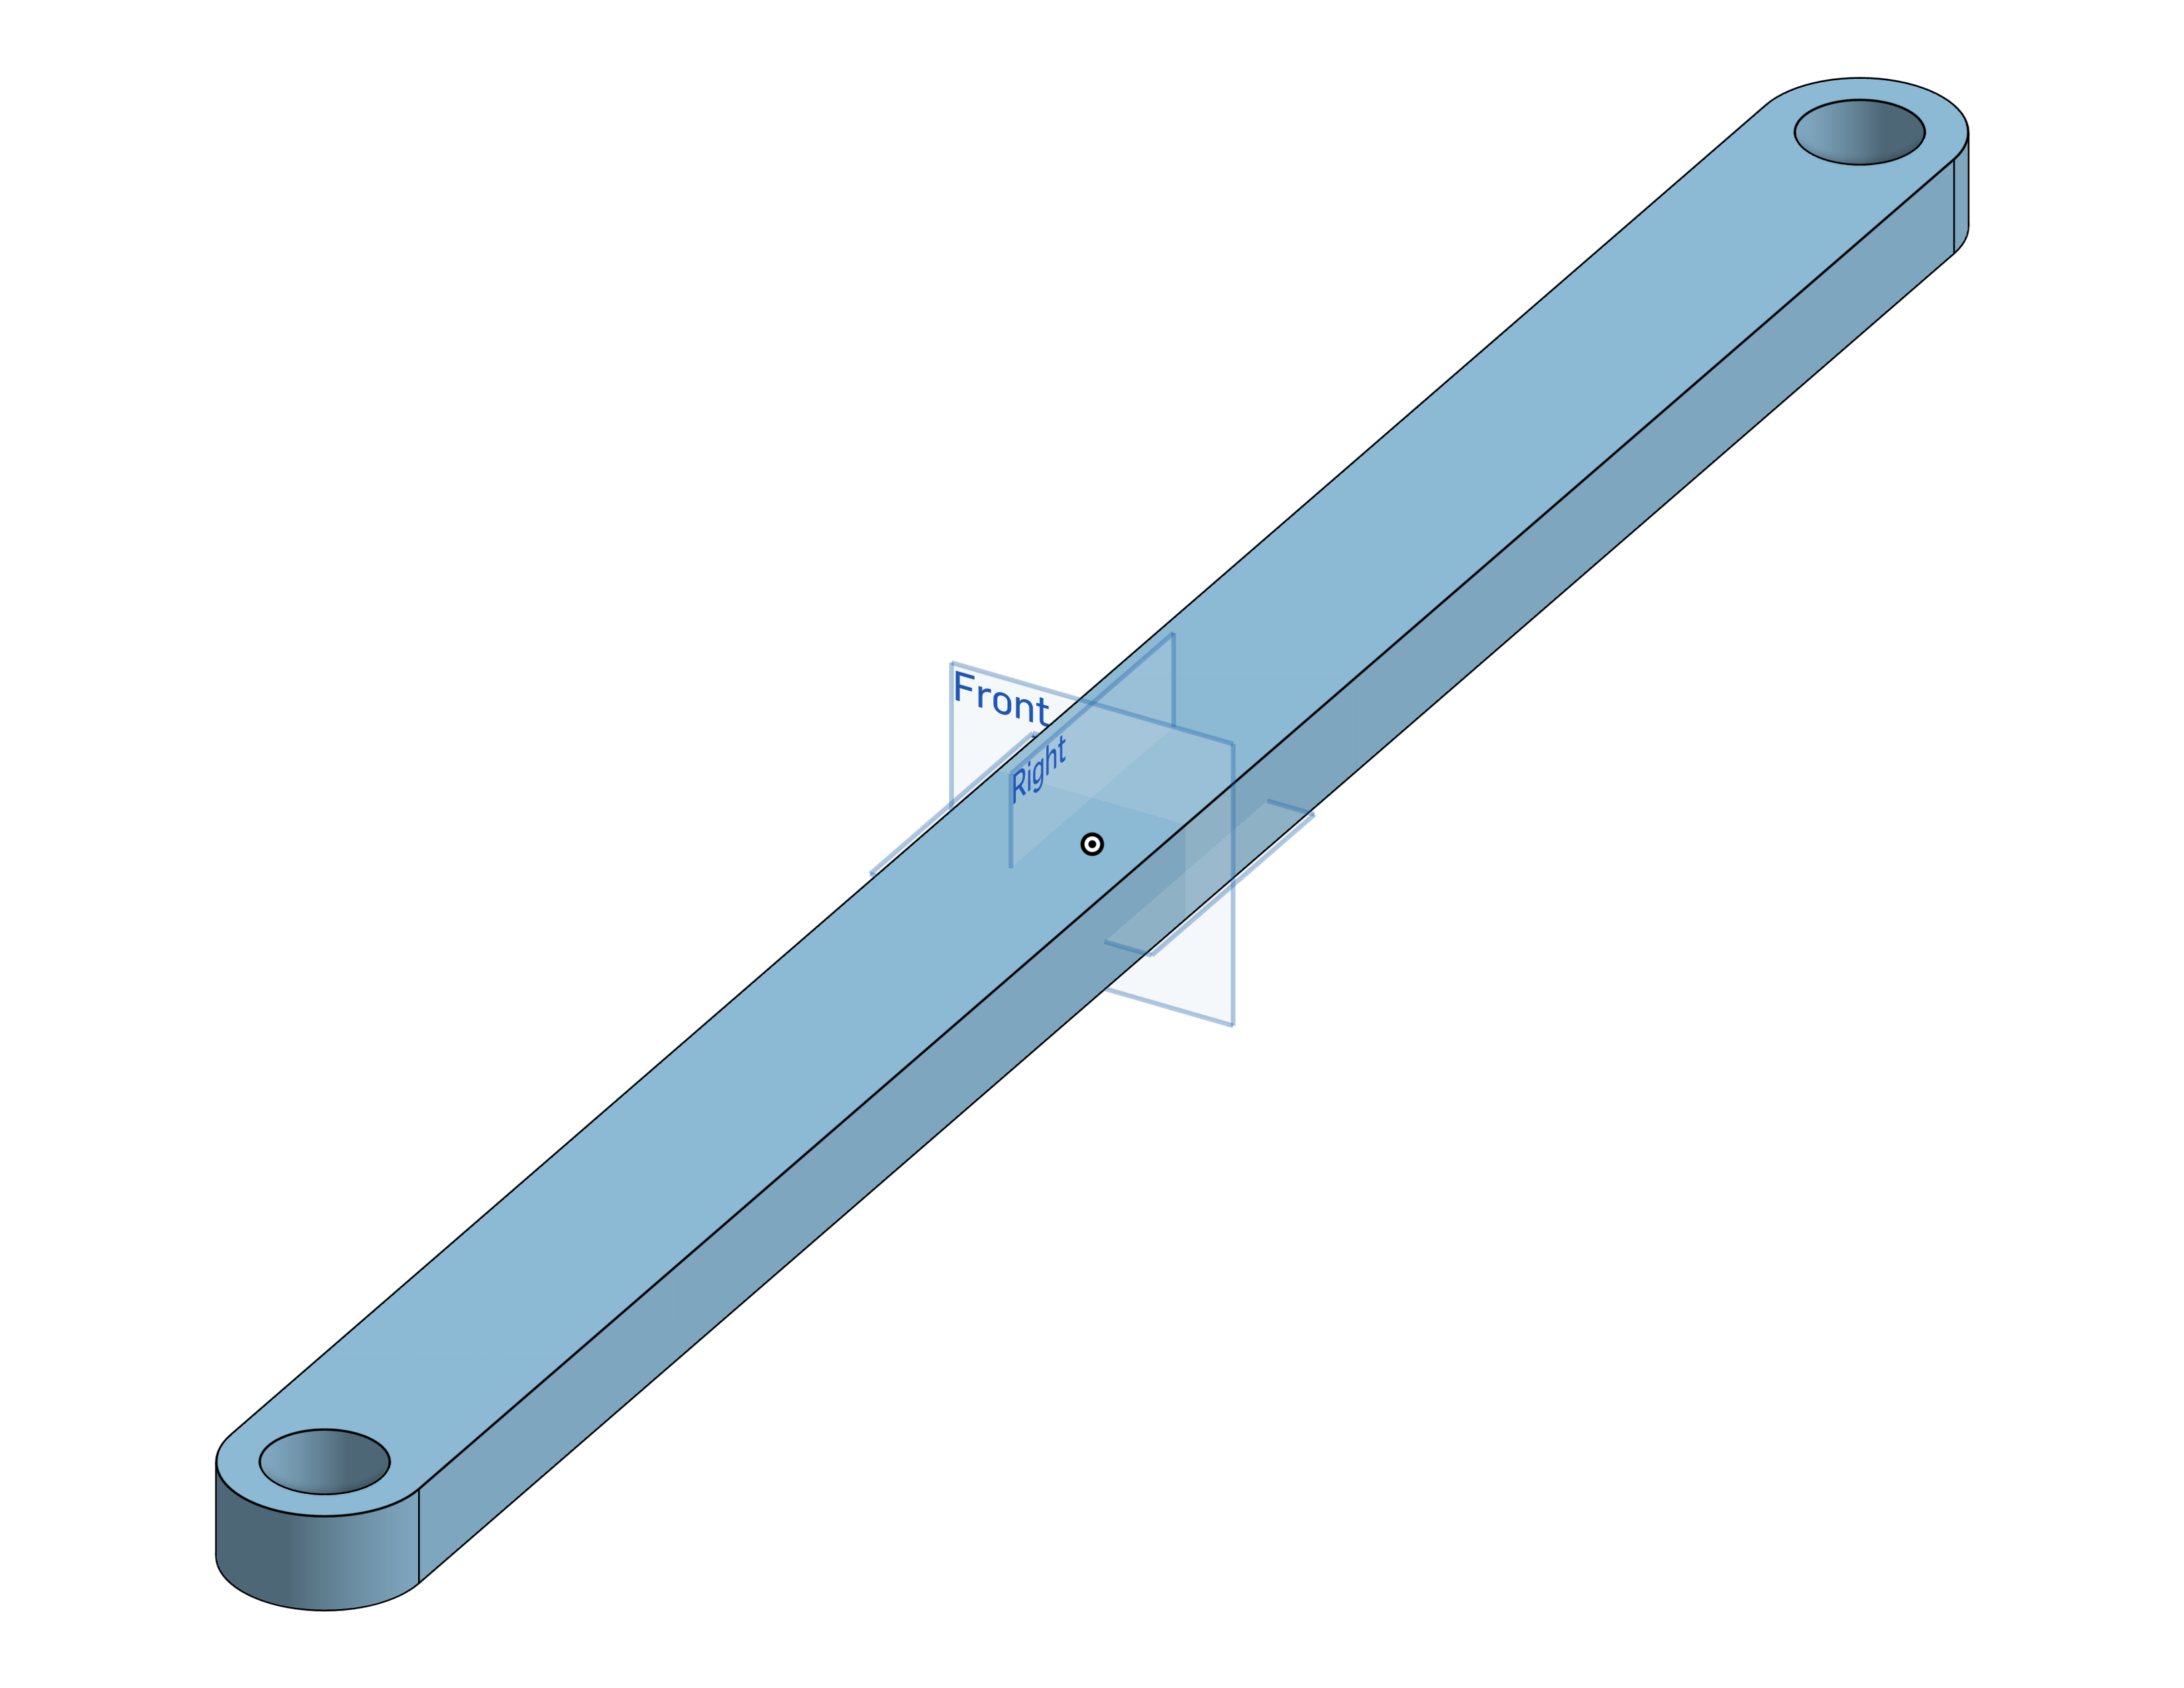
\includegraphics[scale=0.05]{../link-AB-CAD.png}
  \caption{\label{fig:link-AB-CAD}Link AB modeled in Onshape.}
\end{figure}

\begin{table}[H] % put here, requires float package
  \begin{center}
    \begin{tabular}{ c|c }  % | for vertical lines
    Link & Mass (\text{kg})   \\
    \hline % for horizontal lines
    AB & 8.35   \\
    BC & 20.2   \\
    CDE & 34.85   \\
    EF &  16.82  \\
    FG &  62.11  \\
    \end{tabular}
  \end{center}\caption{Link masses.}\label{tab:link-masses}
\end{table}

\subsection{Mass Moment of Inertia Calculations}%
\label{eqns.mmi}

The mass moments of inertia are given by Onshape's ``Mass and Section Properties'' feature mentioned in Section \ref{eqns.masses}, and are shown in Table \ref{tab:link-mmi}. The MMI is about the axis formed by the intersection of the Front and Top planes in Figure \ref{fig:link-AB-CAD}.

\begin{table}[H] % put here, requires float package
  \begin{center}
    \begin{tabular}{ c|c }  % | for vertical lines
      Link & MMI (kg$\cdot$m$^{2}$) \\
      \hline
      AB & 0.266   \\
      BC & 3.53   \\
      CDE & 18.54   \\
      EF & 2.05 \\
      FG & 103 \\
    \end{tabular}
  \end{center}\caption{Link mass moments of inertia.}\label{tab:link-mmi}
\end{table}

\subsection{Kinematics Equations}%
\label{eqns.kinematics}

I developed my kinematic equations from two vector loops: A-B-C-D-A and D-E-F-G-D. Note that these represent two four-bar linkages in series, with ternary link DEC as the common link.

\subsubsection{Position}%
\label{eqns.kinematics.position}

For loop ABCDA, the position loop is:
\[ \vec{r}_{b/a} + \vec{r}_{c/b} + \vec{r}_{d/c} + \vec{r}_{a/d} = 0 \]
For loop DEFGD, the position loop is:
\[ \vec{r}_{e/d} + \vec{r}_{f/e} + \vec{r}_{g/f} + \vec{r}_{d/g} = 0 \]

\subsubsection{Velocity}%
\label{eqns.kinematics.velocity}

Differentiate the positions loop equations to derive the velocity loop equations:
\[ \vec{v}_{b/a} + \vec{v}_{c/b} + \vec{v}_{d/c} + \vec{v}_{a/d} = 0 \]
\[ \vec{v}_{e/d} + \vec{v}_{f/e} + \vec{v}_{g/f} + \vec{v}_{d/g} = 0 \]
The velocity of a joint $j$ relative to $i$ can be decomposed into translational and rotational components:
\[ \vec{v}_{j/i} = \vec{v}_{i} + (\omega_{ij}\times \vec{r}_{j/i}) \]
For a ground joint $i$, $\vec{v}_{i}$ is zero. For joints $i$ and $j$ of the same rigid link, their relative translational velocity is also zero. All joints and links in this linkage satisfy these conditions, so all translational velocity terms are zero for all joints. Therefore, the velocity loop equations for the loop equations reduce to the rotational components:
\[ (\vec{\omega}_{ab}\times \vec{r}_{b/a}) + (\vec{\omega}_{bc}\times \vec{r}_{c/b}) + (\vec{\omega}_{cd}\times \vec{r}_{d/c}) + (\vec{\omega}_{da}\times \vec{r}_{a/d}) = 0 \]
\[ (\vec{\omega}_{de}\times \vec{r}_{e/d}) + (\vec{\omega}_{ef}\times \vec{r}_{f/e}) + (\vec{\omega}_{fg}\times \vec{r}_{g/f}) + (\vec{\omega}_{dg}\times \vec{r}_{g/d}) = 0 \]\\

To solve the loop equations we require the steady-state crank angular velocity, $\omega_{1}$. With a part per hour rate of 7450 parts per seven hours, we can compute:
\[ \dot{p} = \frac{7450 \text{part}}{7 \text{hr}} = 0.29 \frac{\text{part}}{\text{sec}} \]
\[ p^{-1} = 3.38 \frac{\text{s}}{\text{part}} \]
By inspection of the PMKS+ model, we see that the output link completes one cycle at the same rate as the input link. Thus:
\[ \omega_{1} = \omega_{5} \]
The output link delivers one part per revolution, so the output link angular velocity is:
\[ \omega_{5} = \frac{2\pi}{p^{-1}}\cdot \text{1 part}  \]
\[ \Rightarrow \omega_{1} = 1.86 \text{rad}/\text{s} \]

\subsubsection{Acceleration}%
\label{eqns.kinematics.acceleration}

Differentiate the velocity loop equations to derive the acceleration loop equations. Begin by differentiating the general rotational velocity:
\[ \frac{d }{d t} \left( \omega_{j/i}\times \vec{r}_{j/i} \right) = (\vec{\alpha}_{j/i}\times \vec{r}_{j/i}) +  \omega_{j/i}\times (\omega_{j/i}\times \vec{r}_{j/i}) \]
Written compactly, the acceleration loop equations are thus:
\[ \Sigma (\vec{\alpha}_{j/i}\times \vec{r}_{j/i}) +  \omega_{j/i}\times (\omega_{j/i}\times \vec{r}_{j/i}) \text{ for } i,j \cap \{(a,b),(b,c),(c,d),(d,a)\} \]
\[ \Sigma (\vec{\alpha}_{j/i}\times \vec{r}_{j/i}) +  \omega_{j/i}\times (\omega_{j/i}\times \vec{r}_{j/i}) \text{ for } i,j \cap \{(d,e),(e,f),(f,g),(g,d)\} \]

\subsection{Accelerations at COMs}%
\label{eqns.accels}

The acceleration at the center of mass of a link is defined with respect to a grounded joint. For link $ij$ with ground joint $j$:
\[ \vec{a}_{s,ij} \equiv \vec{a}_{s,ij/j} = \vec{\alpha}_{ij} \times \vec{r}_{s,ij/j} + \vec{\omega}_{ij}\times \langle \vec{\omega}_{ij} , \vec{r}_{s,ij/j} \rangle \]
For a non-grounded link $ik$ sharing a joint $i$ with grounded link $ij$, the acceleration must be decomposed relative to $i$ before relative to the ground joint $j$:
\[ \vec{a}_{s,ik} \equiv \vec{a}_{s,ik/j} = \vec{a}_{s,ik/i} + \vec{a}_{i/j} \]
where $\vec{a}_{s,ik/i}$ and $\vec{a}_{i/j}$ are both of the form described above for a grounded joint.

\section{Results}%
\label{res}

\subsection{First Position}%
\label{res.first}

\subsubsection{Joint Forces and Torques}%
\label{res.first.joints}

\subsubsection{Postion, Velocity, and Acceleration}%
\label{res.first.kin}

\subsubsection{Masses and Mass Moments of Inertia}%
\label{res.first.mass-mmi}

\subsection{Plots}%
\label{res.plots}

\subsection{Comparison with PMKS+}%
\label{res.compare}

\subsubsection{Joint Position}%
\label{res.compare.linJointPos}

Comparison of the linear joint positions is shown in Figure \ref{fig:compare.linJointPos}. By inspection, the values are similar, though differences in computational methods yield results that are not exactly equivalent. Positions for ground joints are trivial (joint coordinates).

\begin{figure}[ht]
  \centering
  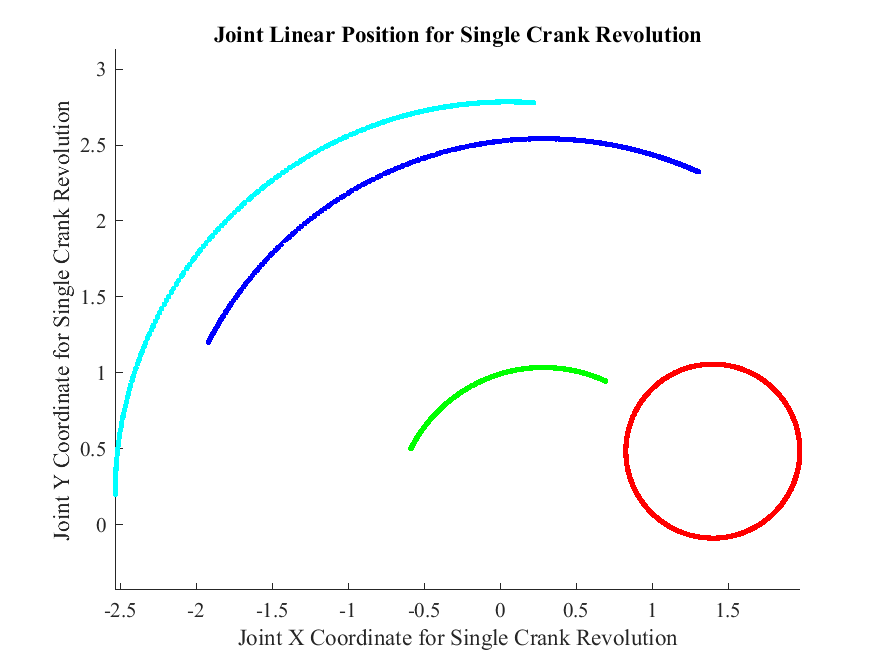
\includegraphics[scale=0.5]{../matlab-plots/linJointPos.png}%
  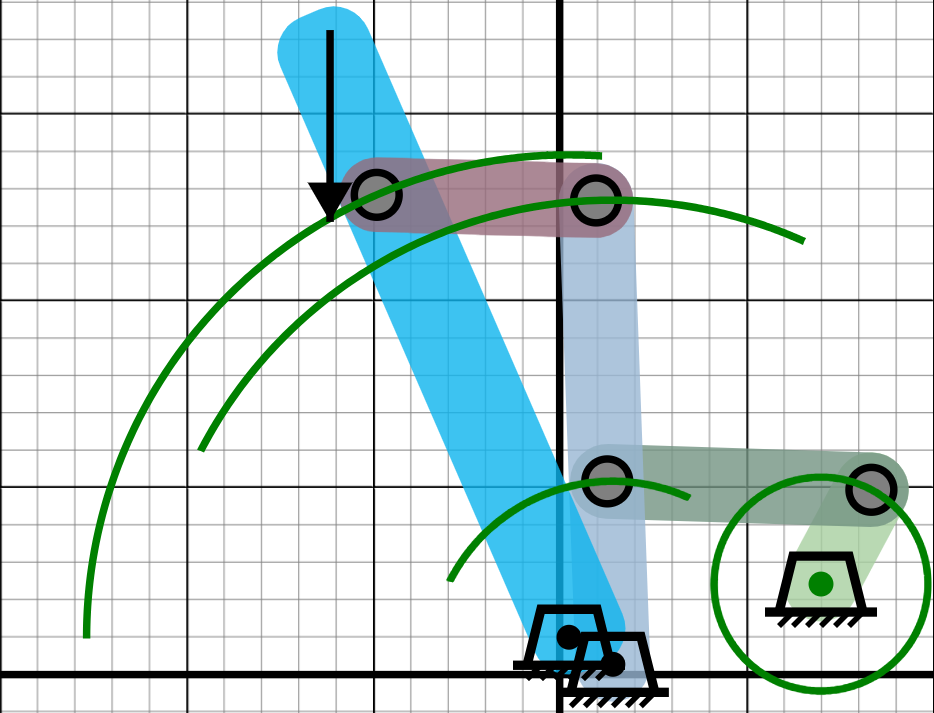
\includegraphics[scale=0.25]{../pmks-plots/linJointPos.png}
  \caption{\label{fig:compare.linJointPos}Linear joint position comparison: my results (left) and PMKS+ (right).}
\end{figure}

\subsubsection{Joint Velocity}%
\label{res.compare.linJointVel}

Comparison of the linear joint velocities is shown in Figure \ref{fig:compare.linJointVel}. By inspection, the values are similar, though differences in computational methods yield results that are not exactly equivalent. Velocities for ground joints are trivial (zero).

\begin{figure}[ht]
  \centering
  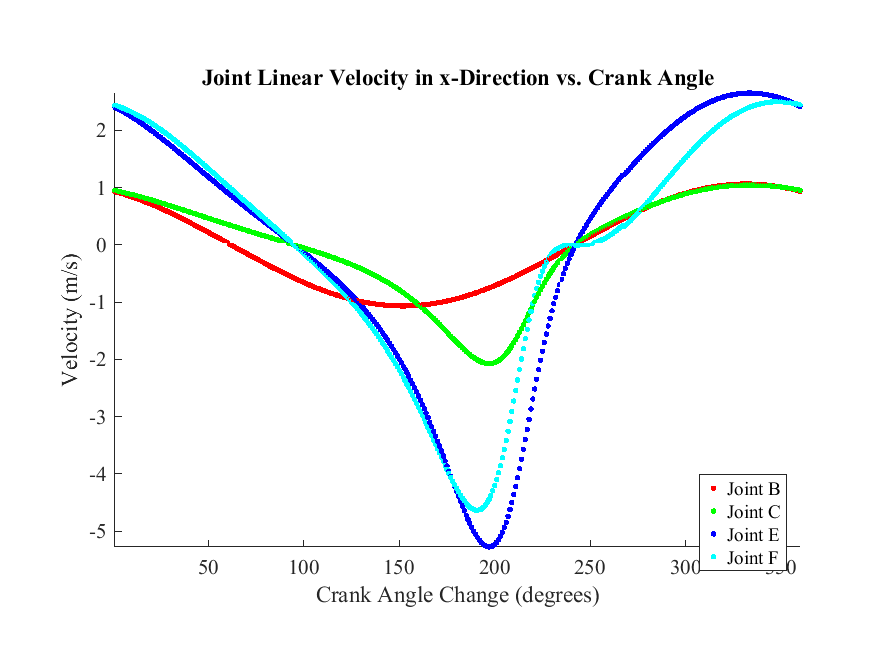
\includegraphics[scale=0.5]{../matlab-plots/linJointVelX.png}%
  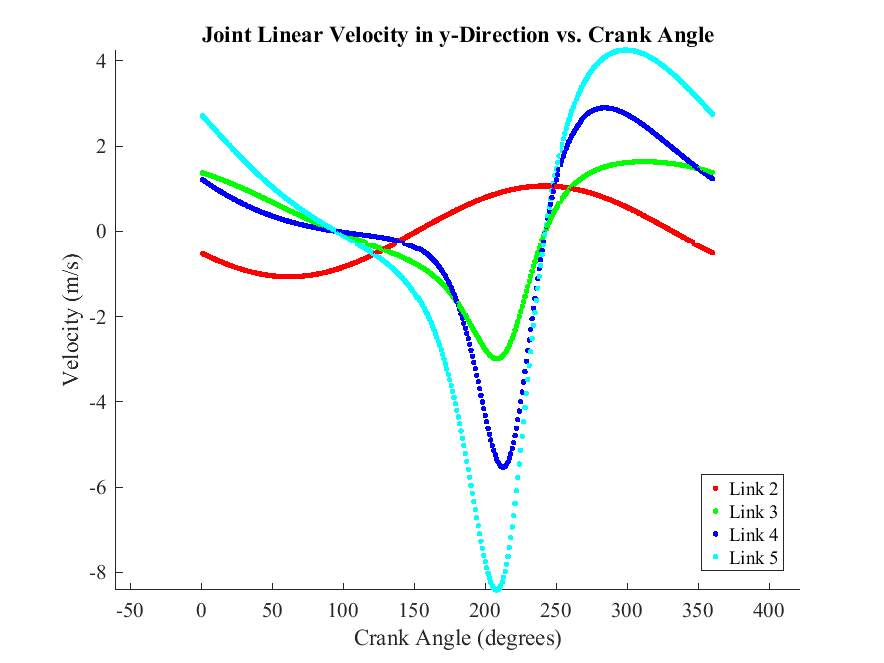
\includegraphics[scale=0.5]{../matlab-plots/linJointVelY.png}\\

  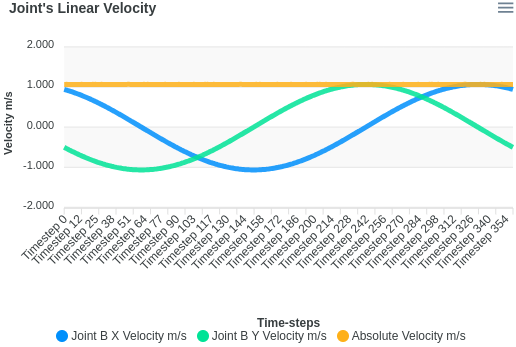
\includegraphics[scale=0.45]{../pmks-plots/linJointVel/linJointVelB.png}%
  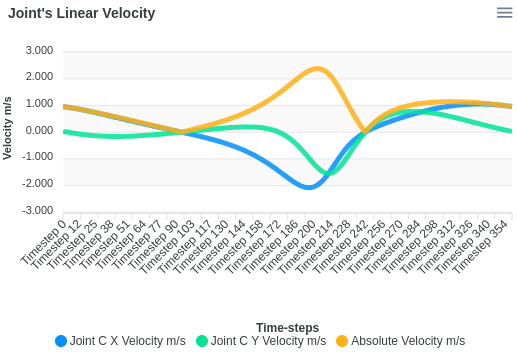
\includegraphics[scale=0.45]{../pmks-plots/linJointVel/linJointVelC.png}

  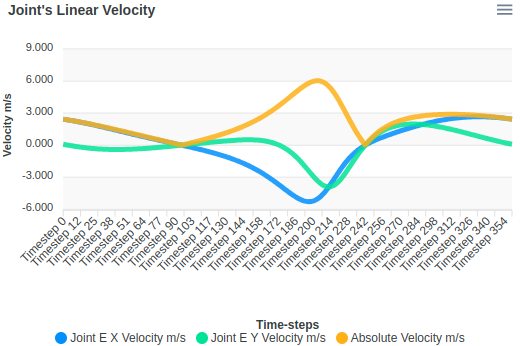
\includegraphics[scale=0.45]{../pmks-plots/linJointVel/linJointVelE.png}%
  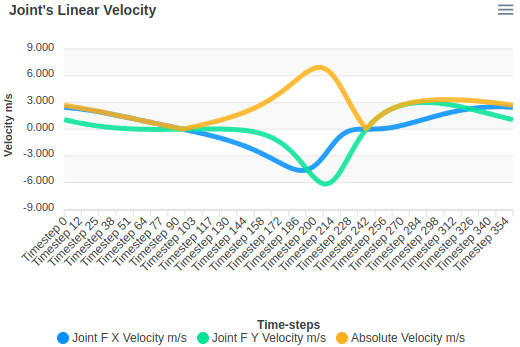
\includegraphics[scale=0.45]{../pmks-plots/linJointVel/linJointVelF.png}%
  \caption{\label{fig:compare.linJointVel}Linear joint velocity comparison: my results (above) and PMKS+ (below).}
\end{figure}

\subsubsection{Joint Acceleration}%
\label{res.compare.linJointAcc}

Comparison of the joint accelerations is shown in Figure \ref{fig:compare.linJointAcc}. By inspection, the values are similar, though differences in computational methods yield results that are not exactly equivalent. Accelerations for ground joints are trivial (zero).

\begin{figure}[ht]
  \centering
  % \includegraphics[scale=0.5]{../matlab-plots/linJointAccX.png}%
  % \includegraphics[scale=0.5]{../matlab-plots/linJointAccY.png}\\

  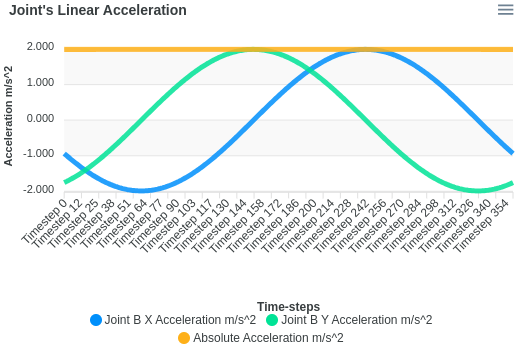
\includegraphics[scale=0.45]{../pmks-plots/linJointAcc/linJointAccB.png}%
  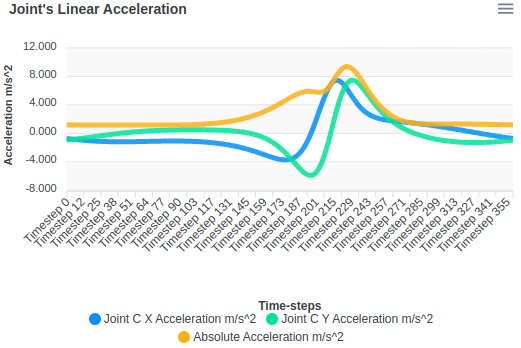
\includegraphics[scale=0.45]{../pmks-plots/linJointAcc/linJointAccC.png}

  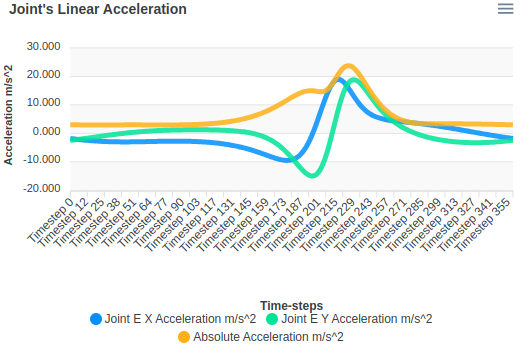
\includegraphics[scale=0.45]{../pmks-plots/linJointAcc/linJointAccE.png}%
  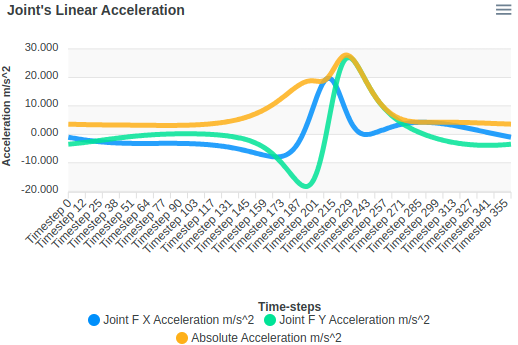
\includegraphics[scale=0.45]{../pmks-plots/linJointAcc/linJointAccF.png}%
  \caption{\label{fig:compare.linJointAcc}Linear joint acceleration comparison: my results (above) and PMKS+ (below).}
\end{figure}

\subsubsection{Link Angular Velocity}%
\label{res.compare.angLinkVel}

Comparison of the link angular velocity is shown in Figure \ref{fig:compare.angLinkVel}. By inspection, the values are similar, though differences in computational methods yield results that are not exactly equivalent. Angular velocity for the crank is trivial ($\omega_{\text{in}}$).

\begin{figure}[ht]
  \centering
  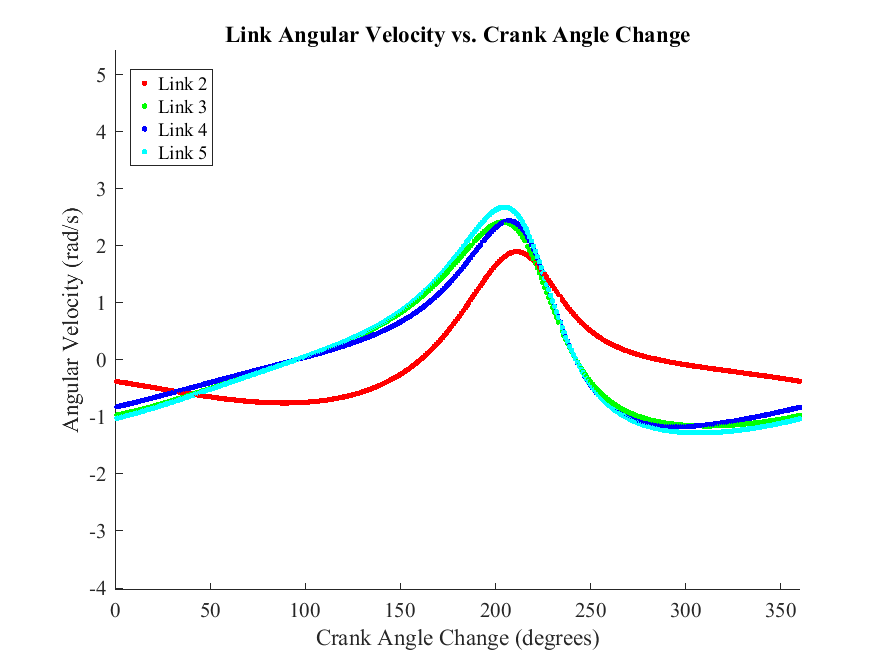
\includegraphics[scale=0.5]{../matlab-plots/angLinkVel.png}

  BC 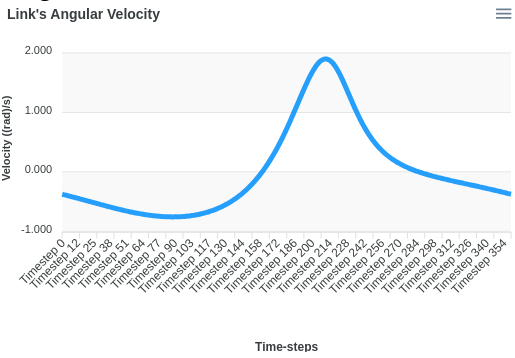
\includegraphics[scale=0.4]{../pmks-plots/angLinkVel/angLinkVelCB.png}%
  CDE 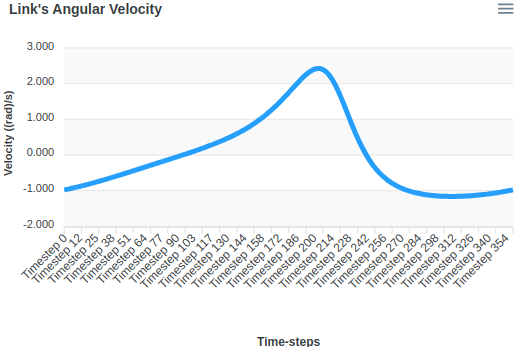
\includegraphics[scale=0.4]{../pmks-plots/angLinkVel/angLinkVelCDE.png}

  EF 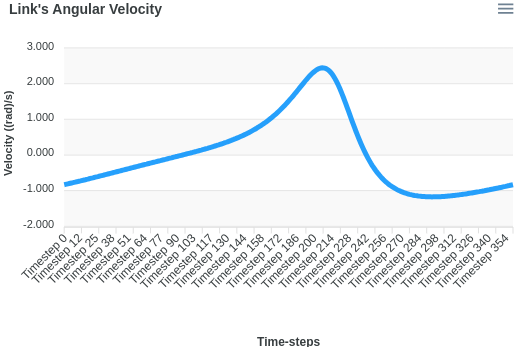
\includegraphics[scale=0.4]{../pmks-plots/angLinkVel/angLinkVelEF.png}%
  FG 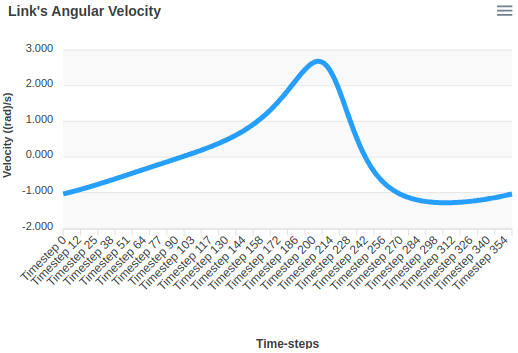
\includegraphics[scale=0.4]{../pmks-plots/angLinkVel/angLinkVelFG.png}%
  \caption{\label{fig:compare.angLinkVel}Link angular velocity comparison: my results (above) and PMKS+ (below).}
\end{figure}

\subsubsection{Link Angular Acceleration}%
\label{res.compare.angLinkAcc}

Comparison of the link angular acceleration is shown in Figure \ref{fig:compare.angLinkAcc}. By inspection, the values are similar, though differences in computational methods yield results that are not exactly equivalent. Angular acceleration for the crank is trivial (zero).

\begin{figure}[ht]
  \centering
  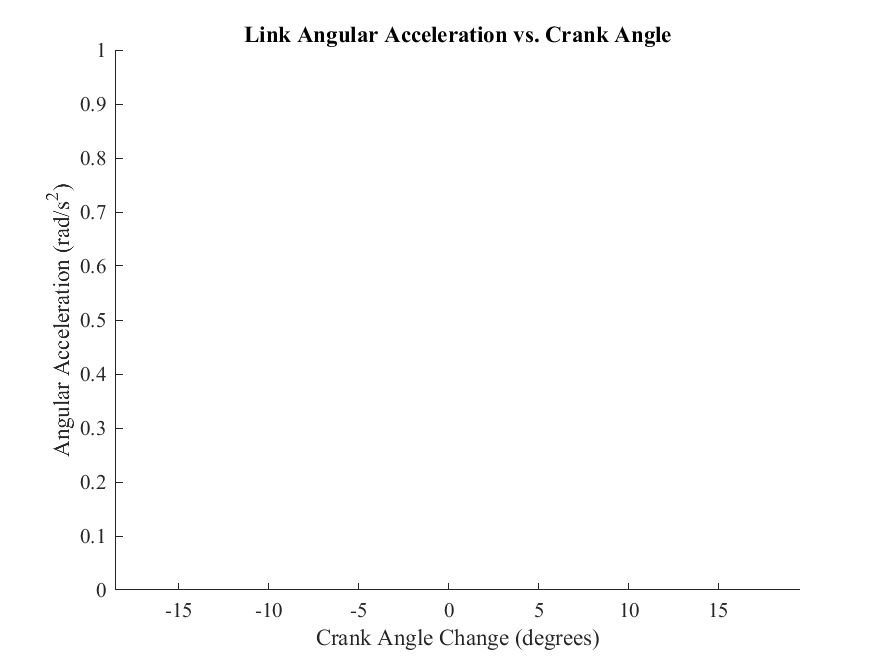
\includegraphics[scale=0.5]{../matlab-plots/angLinkAccel.png}

  BC 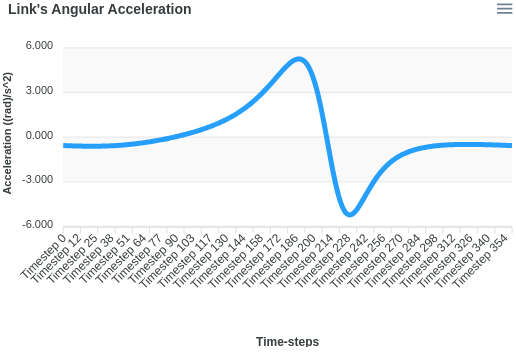
\includegraphics[scale=0.4]{../pmks-plots/angLinkAcc/angLinkAccBC.png}%
  CDE 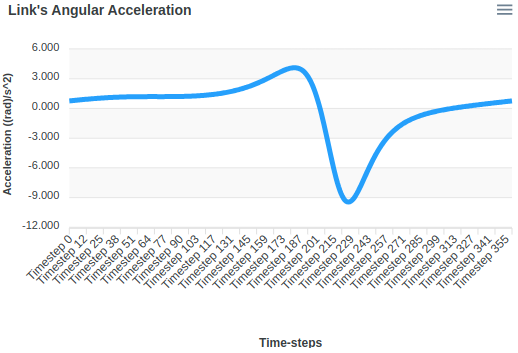
\includegraphics[scale=0.4]{../pmks-plots/angLinkAcc/angLinkAccCDE.png}

  EF 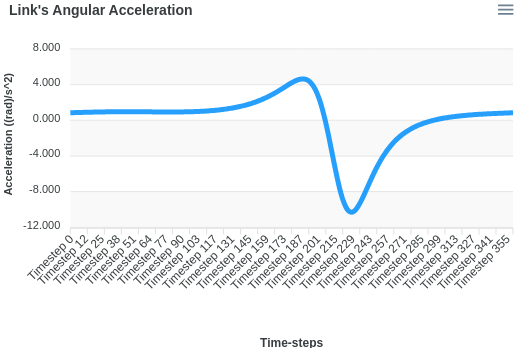
\includegraphics[scale=0.4]{../pmks-plots/angLinkAcc/angLinkAccEF.png}%
  FG 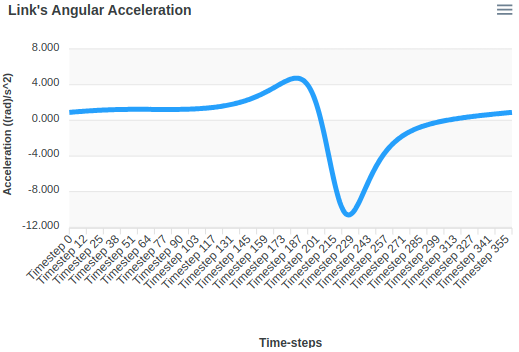
\includegraphics[scale=0.4]{../pmks-plots/angLinkAcc/angLinkAccFG.png}%
  \caption{\label{fig:compare.angLinkAcc}Link angular acceleration comparison: my results (above) and PMKS+ (below).}
\end{figure}


\section{MATLAB Code}%
\label{code}

I have employed object-oriented programming to manage state across a single event loop for computing dynamic kinematic and kinetic variables. The \texttt{Link} and \texttt{Joint} classes form the basic elements of the linkage, and the \texttt{Linkage} class is instantiated a single time and comprises the linkage itself. Given that I have not ended up abstracting further into classes such as \texttt{TernaryLink} and implementing functionality to, for example, define kinematic loops, many hacks and inefficiencies are present in this program. Coding this was quite interesting, as it got me thinking about the real-time, mechanical state of an entire linkage. This was also more exciting than having a bunch of structs and independent scripts.

This entire report, its code, and media like photos and plots are all stored at this Github repository: \href{https://github.com/lorenzohess/ME-4322-Linkage-Homework}{github.com/lorenzohess/ME-4322-Linkage-Homework}. To run the program, invoke \texttt{linkage\_analysis.m}. Note that this script presumes a certain folder hierarchy, so simply downloading the script (even with associated classes) will not necessarily work. This code works on Arch Linux, and although untested on Windows and Mac, should work out of the box. The simulation takes about 5 minutes to run, with some of that time devoted to generating images from plots.

\subsection{\texttt{linkage\_analysis.m}}%

\subsection{\texttt{Linkage.m}}%

\subsection{\texttt{Link.m}}%

\subsection{\texttt{Crank.m}}%

\subsection{\texttt{Joint.m}}%

\subsection{\texttt{compute\_coords.m}}%

\section{Discussion}%
\label{discuss}

\section{References}%
\label{ref}

\end{document}
